%%%% PROCESAR con PdfLaTeX !!!!!


\documentclass[12pt]{book}
\usepackage{geometry}\geometry{top=2cm,bottom=2cm,left=3cm,right=3cm}
\usepackage{amssymb}
\usepackage{amsmath}
\usepackage{graphicx}
\usepackage{txfonts}




\begin{document}
\thispagestyle{empty}

\begin {center}

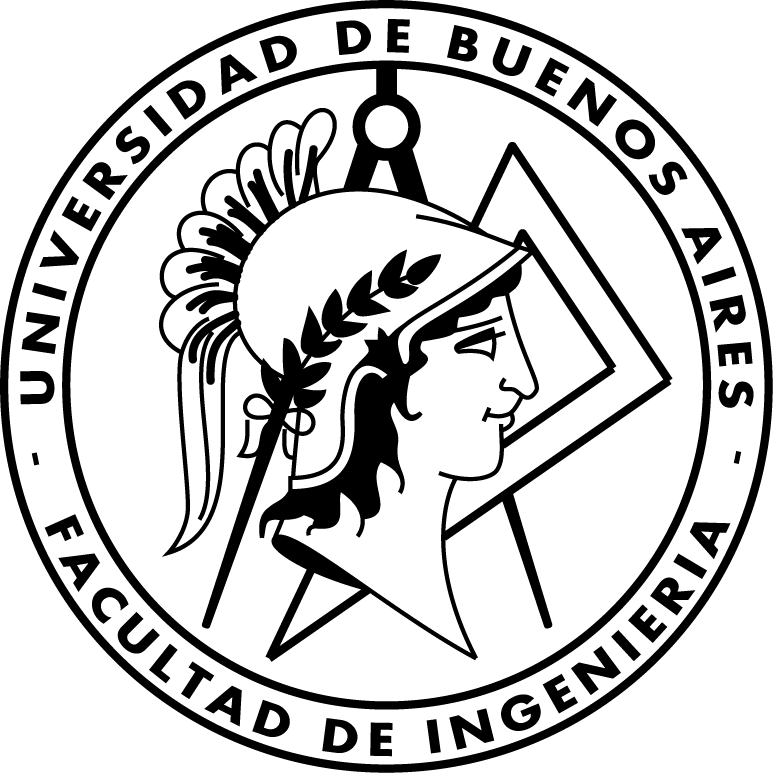
\includegraphics[scale=.4]{Logo-fiuba_big.png}

\medskip
UNIVERSIDAD DE BUENOS AIRES

Ciclo B\'asico Com\'un

\vspace{3cm}

\textbf{\large Introducci\'on a la F\'isica}

\vspace{2cm}


Este es un modesto aporte para los alumnos de la f\'acultad de ingenier\'ia  de la UBA de las carreras de licenciatura en an\'alsis de sistemas e ingenier\'ia inform\'atica.
De ninguna man\'era pretende ser una gu\'ia de estudio, ni remplaza las clases presenciales, el material oficial de la catedra esta disponible en el web site de la m\'ateria.
\\
http://materias.fi.uba.ar/7510/

\end {center}


\vspace{2.5cm}

\noindent Autor:\,	Isaac Edgar Camacho Ocampo
 
\noindent Carrera:\,	Licenciatura en An\'alisis de sistemas

\vspace{1cm}

\vspace{1cm}

\noindent Buenos Aires, 2019

\newpage


\tableofcontents

\tableofcontents
\chapter{Introducción}
\section{Conocimientos previos}
\section{Estado del arte}
\chapter{CINEMATICA}
\section{MRU ( Movimiento Rectilíneo y Uniforme )}
\subsection{Posición, velocidad y aceleración}
\subsection{Sistema de referencia. Trayectoria}
\subsection{Movimiento Rectilíneo y Uniforme}
\subsection{Velocidad en el MRU}
\subsection{Ecuaciones horarias en el MRU}
\subsection{Tg de un ángulo y pendiente de una recta}
\subsection{Gráficos en el MRU}
\subsection{Pendientes y las áreas de los gráficos}
\subsection{Un ejemplo de MRU}
\subsection{Velocidad media}

\section{Teoría clásica}
\subsection{Definición de variables}
\subsection{Pruebas y refutaciones}
\section{Hipótesis}
\chapter{Resultados}
\section{Simulación de resultados}
\subsection{Suposiciones}
\subsection{Modelos}
\section{Resultados preliminares}
\section{Resultados postprocesados}
\subsection{Valores atípicos}
\subsection{Correlaciones}
\chapter{Conclusiones}
\end{document}
